\subsection{Curve in funzione della pressione}
\FloatBarrier
Sono state registrate le posizioni dei centroidi e l'RMS dei picchi in energia e dei picchi di vmax delle alfa delle sorgenti.

\begin{tabella}
 \centering
 \begin{center}
\begin{tabulary}{\textwidth}{CCC}
\toprule
p($mb$) &  posizione centroide & RMS \\ 
650 & 6552$\pm$ 6 & 81$\pm$ 4 \\
600 & 6531$\pm$ 1 & 44 $\pm$1 \\
550 & 6542$\pm$ 2 & 56 $\pm$1 \\
500 & 6531$\pm$ 2 & 65 $\pm$2 \\
450 & 6547$\pm$ 2 & 61 $\pm$1 \\
400 & 6524$\pm$ 2 & 62 $\pm$1 \\
380 & 6495$\pm$ 4 & 63 $\pm$3 \\


 \bottomrule
\end{tabulary}
\end{center}
 
 \caption{Dati picchi in energia e RMS}
 \label{tab:tab_integral1.tex}
\end{tabella}

\begin{tabella}
 \centering
 \begin{center}
\begin{tabulary}{\textwidth}{CCC}
\toprule
p($mb$) &  posizione centroide & RMS \\
650 &6969 $\pm$4.194 &61.64$\pm$ 2.966\\
600 &6951 $\pm$1.737 &48.47$\pm$ 1.228\\
550 &6968 $\pm$2.171 &62.44$\pm$ 1.535\\
500 &6946 $\pm$1.848 &54.53$\pm$ 1.306\\
450 &6966 $\pm$2.233 &64.44$\pm$ 1.579\\
400 &6903 $\pm$2.473 &86.79$\pm$ 1.748\\
380 &6770 $\pm$5.797 &84.21$\pm$ 4.099\\
\bottomrule
\end{tabulary}
\end{center} 
 \caption{Dati picchi in energia e RMS}
 \label{tab:tab_integral2.tex}
\end{tabella}

\begin{tabella}
 \centering
 
\begin{center}
\begin{tabulary}{\textwidth}{CCC}
\toprule
p($mb$) & posizione centroide & RMS \\ 
650 &7372 $\pm$5 &62$\pm$ 4\\
600 &7352 $\pm$2 &44$\pm$ 1\\
550 &7370$\pm$ 2 &56$\pm$ 2\\
500 &7336$\pm$ 2 &54$\pm$ 2\\
450 &7350$\pm$ 3 &65$\pm$ 2\\
\bottomrule
\end{tabulary}
\end{center}
 
 \caption{Dati picchi in energia e RMS}
 \label{tab:tab_integral3.tex}
\end{tabella}

\begin{tabella}
 \centering
 \begin{center}
\begin{tabulary}{\textwidth}{CCC}
\toprule
p($mb$) &  posizione centroide & RMS \\ 
650 &189.3$\pm$ 0.1142& 2.697$\pm$ 0.08075\\
600 &176.8$\pm$ 0.0564& 2.692$\pm$ 0.03988\\
550 &156.4$\pm$ 0.0616& 3.04 $\pm$0.0435\\
500 &144.2$\pm$ 0.05632& 2.803 $\pm$0.03983\\
450 &133.2$\pm$ 0.0983 &5.124 $\pm$0.0694\\
400 &124$\pm$ 0.06664 &3.285 $\pm$0.04712\\
380 &122.9$\pm$ 0.1359& 3.119$\pm$ 0.09609\\
\bottomrule
\end{tabulary}
\end{center} 
 \caption{Dati vmax in emergia e RMS}
 \label{tab:tab_vmax.tex}
\end{tabella}




In seguito sono stati riportati in grafico i centroidi delle energie e i centroidi dei massimi in funzione della pressione:

\begin{grafico}
 \centering
 \resizebox{\textwidth}{!}{%
 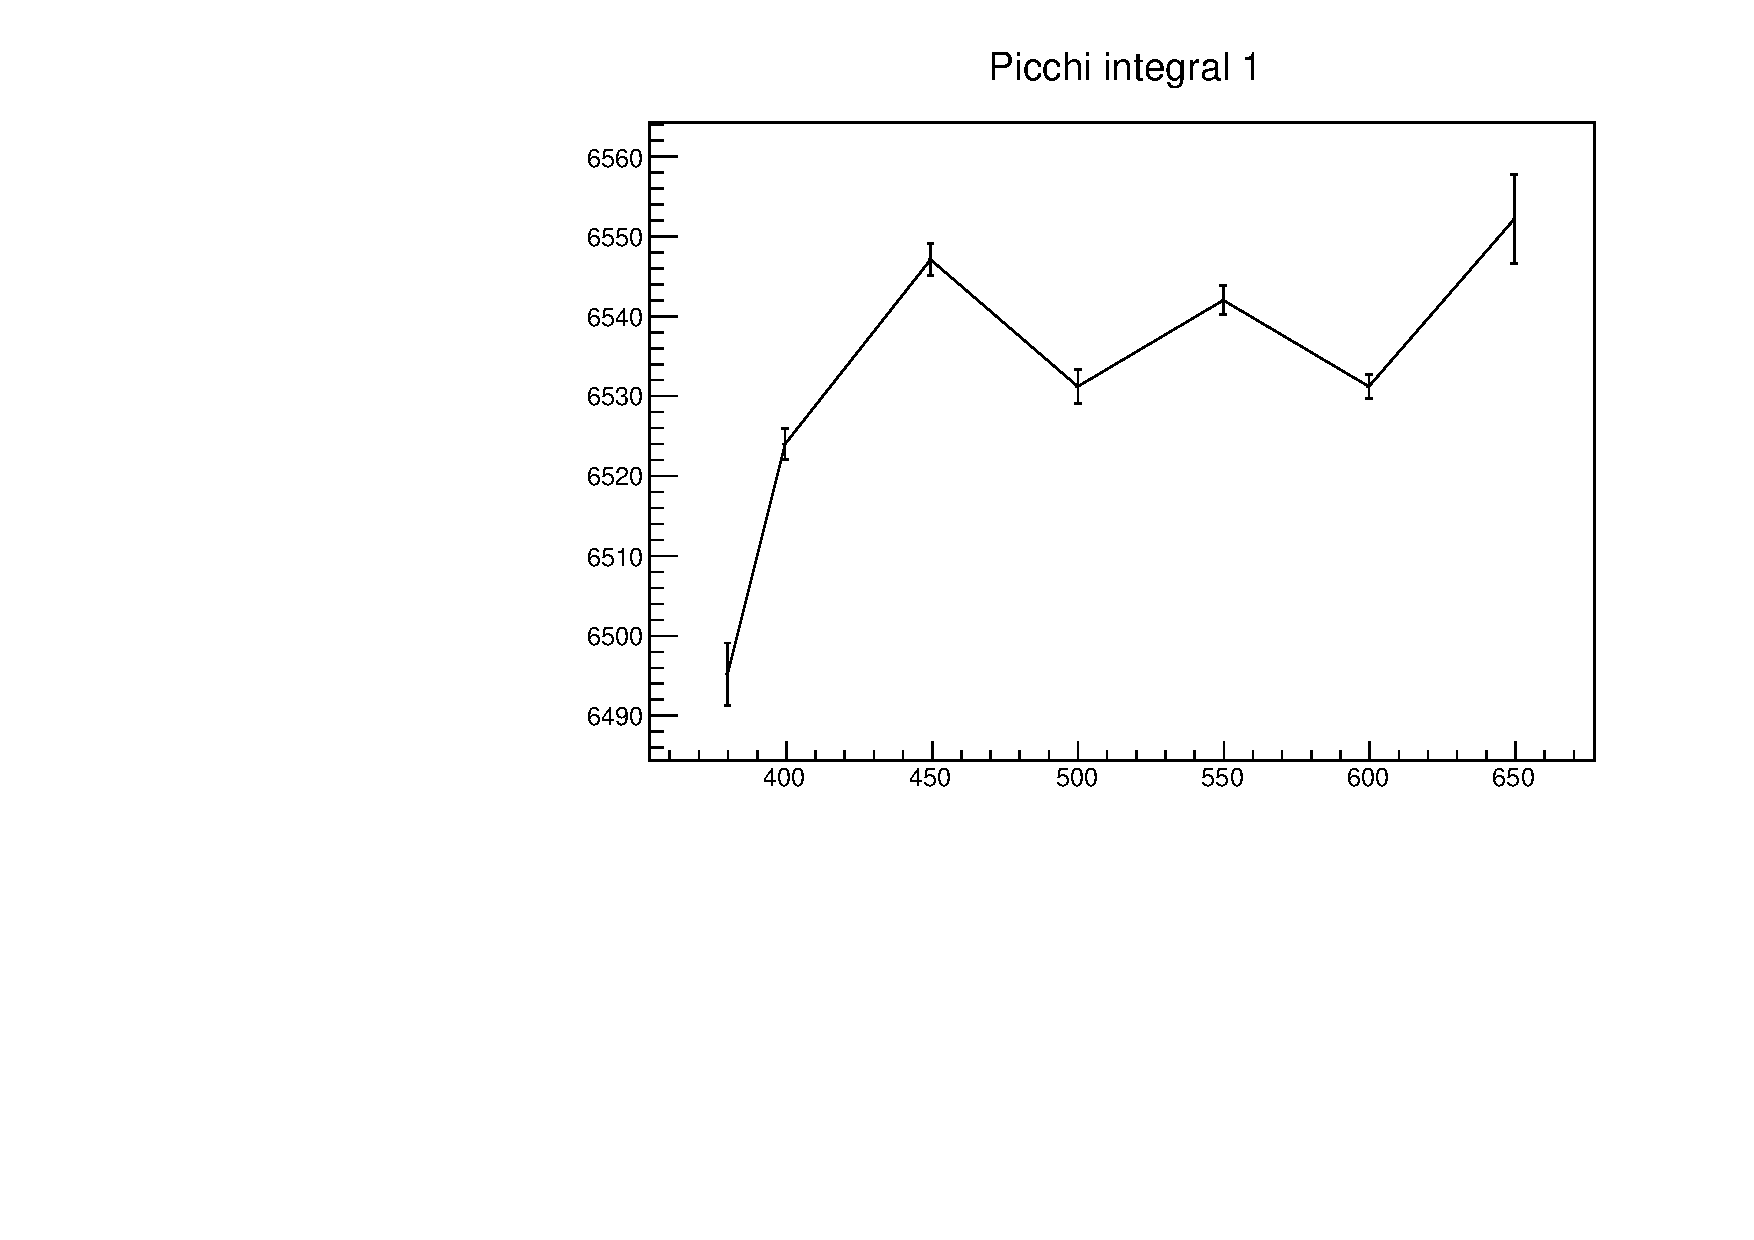
\includegraphics{../grafici/risultati/picchi_integral1.pdf}
 }%
 \caption{Andamento integrale del picco 1 in funzione della pressione [mb]} 
 \label{gr:picchi_int1} 
\end{grafico}

\begin{grafico}
 \centering
 \resizebox{\textwidth}{!}{%
 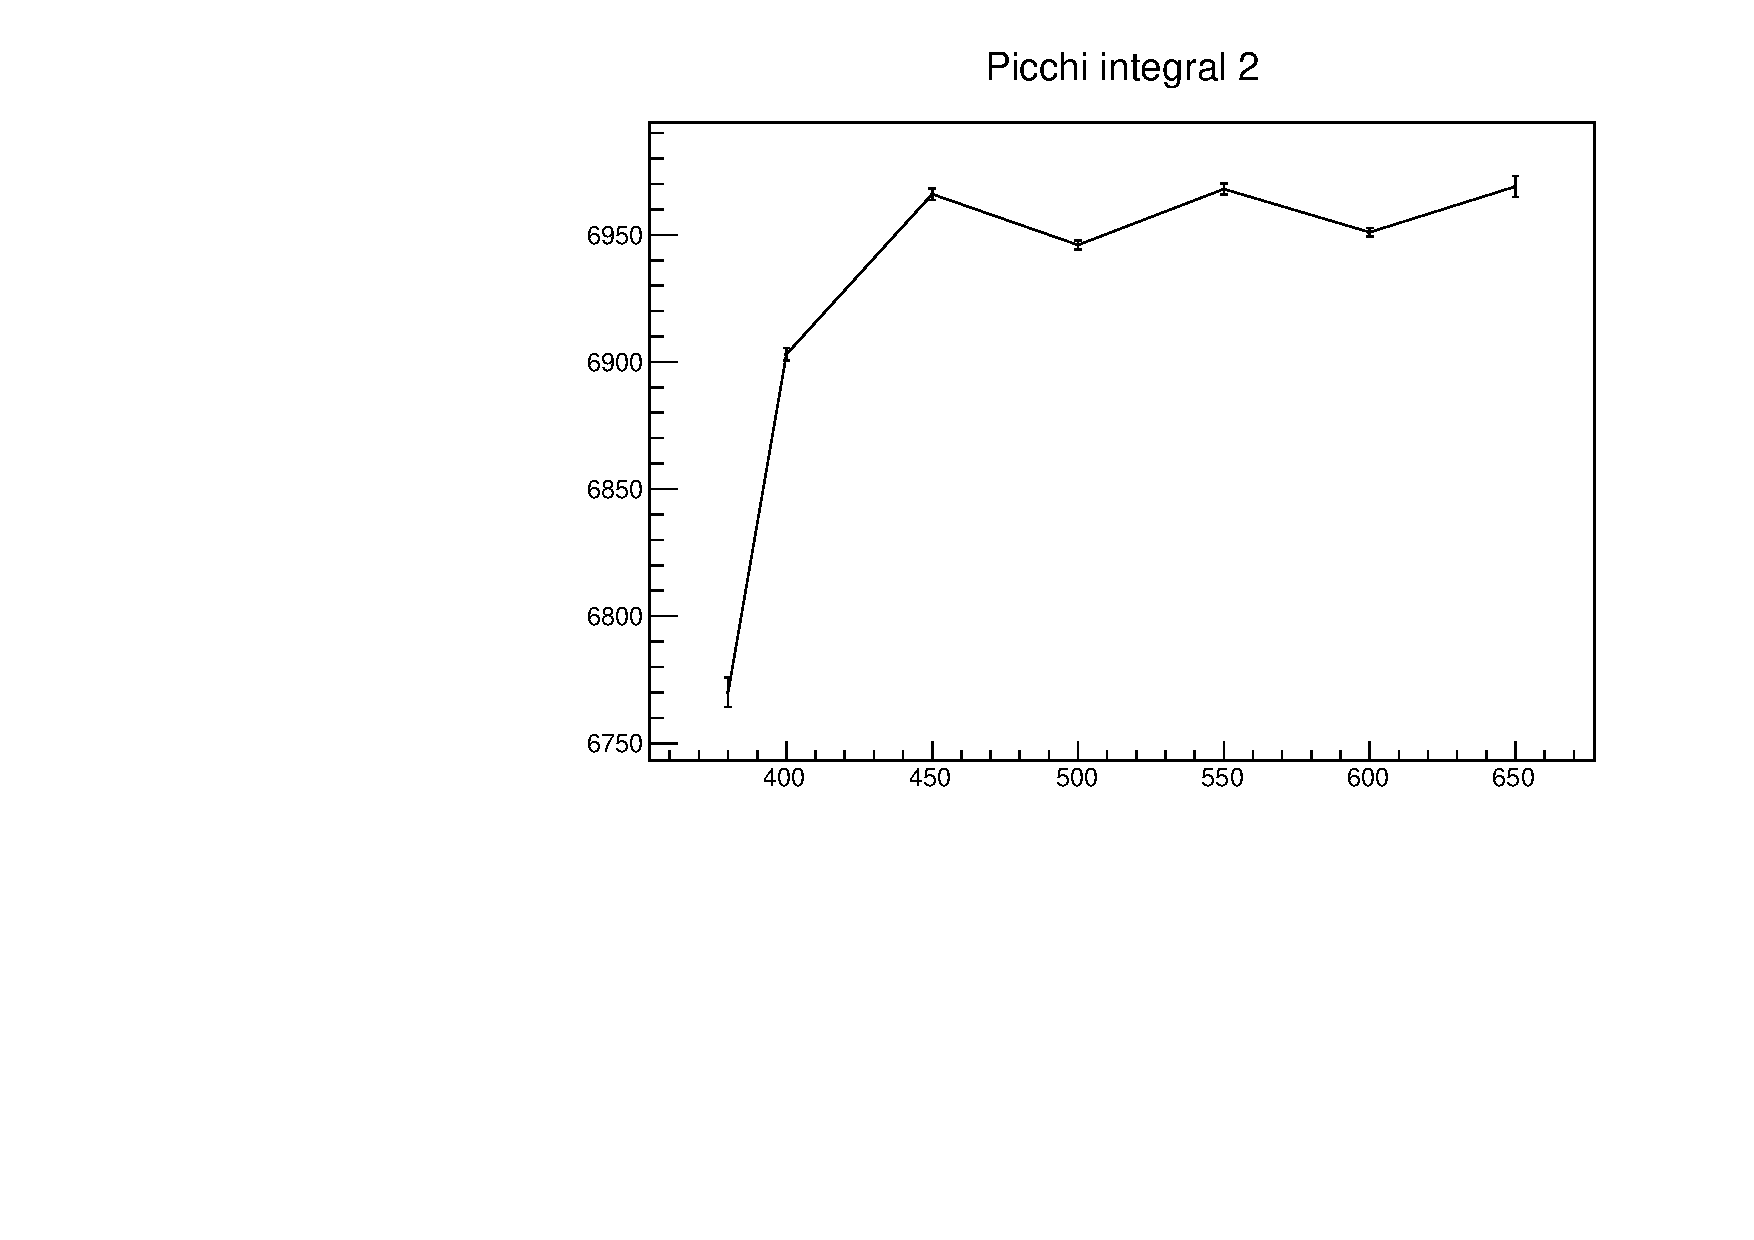
\includegraphics{../grafici/risultati/picchi_integral2.pdf}
 }%
 \caption{Andamento integrale del picco 2 in funzione della pressione [mb]} 
 \label{gr:picchi_int2} 
\end{grafico}

\begin{grafico}
 \centering
 \resizebox{\textwidth}{!}{%
 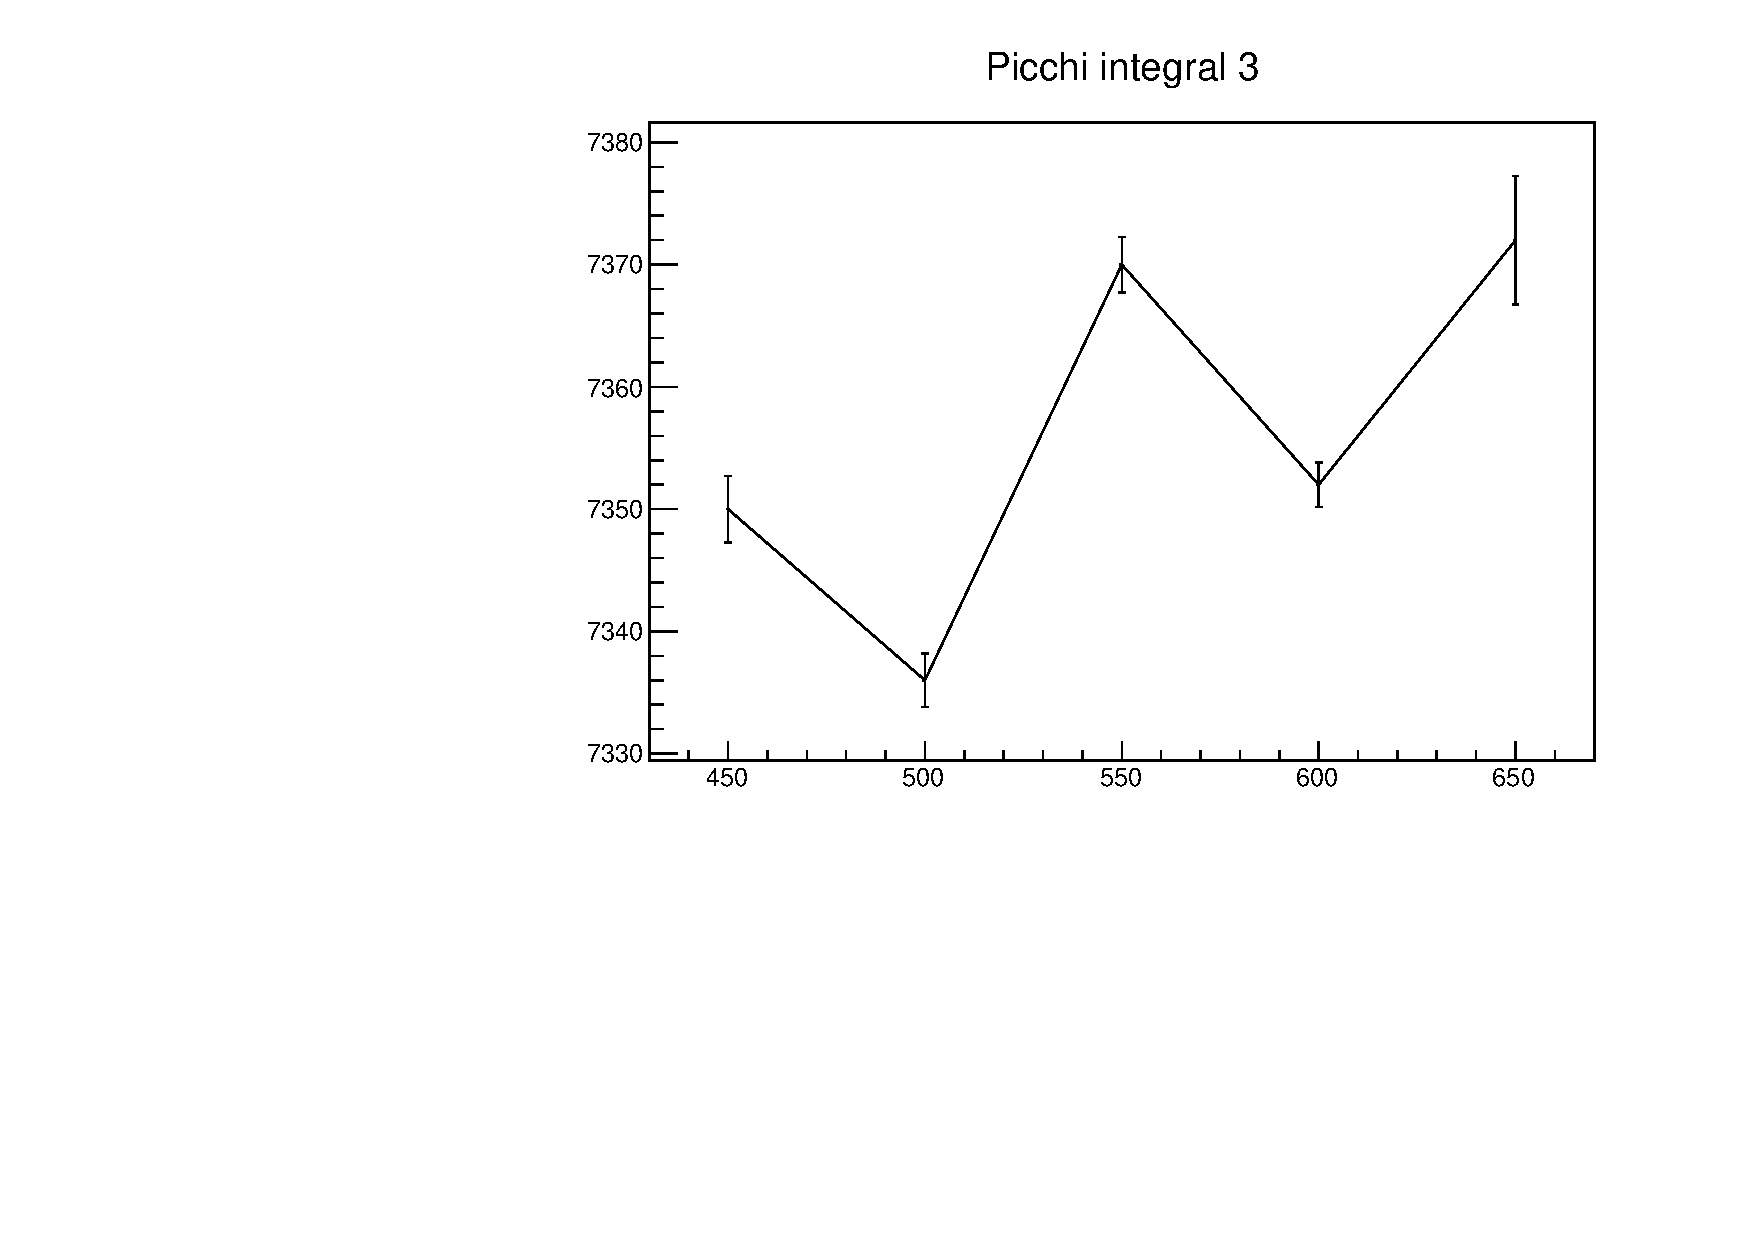
\includegraphics{../grafici/risultati/picchi_integral3.pdf}
 }%
 \caption{Andamento integrale del picco 3 in funzione della pressione [mb]} 
 \label{gr:picchi_int3} 
\end{grafico}

\begin{grafico}
 \centering
 \resizebox{\textwidth}{!}{%
 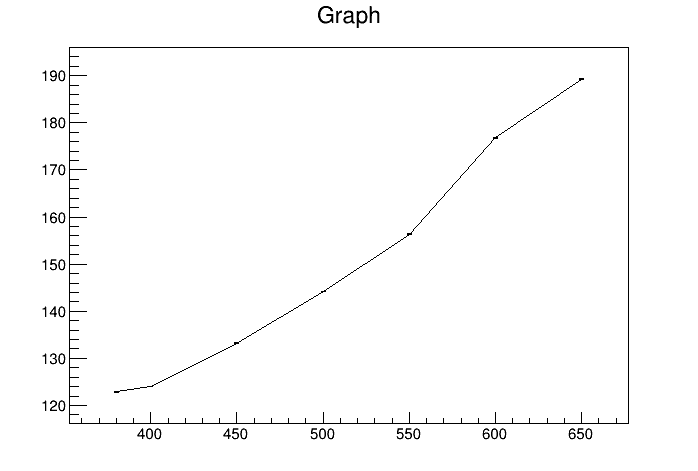
\includegraphics{../grafici/risultati/picchi_vmax.png}
 }%
 \caption{Andamento integrale di vmax [V] in funzione della pressione [mb]} 
 \label{gr:picchi_vmax} 
\end{grafico}

Come si può vedere dai grafici 	\autoref{gr:picchi_int1}, \autoref{gr:picchi_int2} e \autoref{gr:picchi_int3}, l'integrale dei picchi, ovvero l'energia della particella alfa, rimane costante al variare della pressione,
almeno finche non si arriva a pressioni troppo basse. Questo cambiamento a pressioni basse è dovuto al fatto che a bassa pressione le particelle riescono ad arrivare oltre la lunghezza della camera, e la restante carica non viene più rivelata.
Addirittura, il terzo picco sparisce a basse pressioni, confondendosi con il secondo a causa dell'energia mancante.

Nel grafico \autoref{gr:picchi_vmax} invece si può chiaramente notare un andamento crescente, dovuto alla dipendenza dalla densità della perdita di energia ($\rho\propto p$).

\FloatBarrier